\begin{block}{one size doesn't fit all!}
    \begin{itemize}
        \item Tailoring guidance to specific building characteristics can improve outcomes
        \item Elevating to ``\gls{bfe} plus a foot'' is not always optimal \cite{xian_elevation:2017,zarekarizi_suboptimal:2020}
        \item Both over- and under-building can be costly \cite{ansar_bigisfragile:2017,DossGollin:2019}
    \end{itemize}
    \begin{framed}
        \begin{figure}
            \centering
            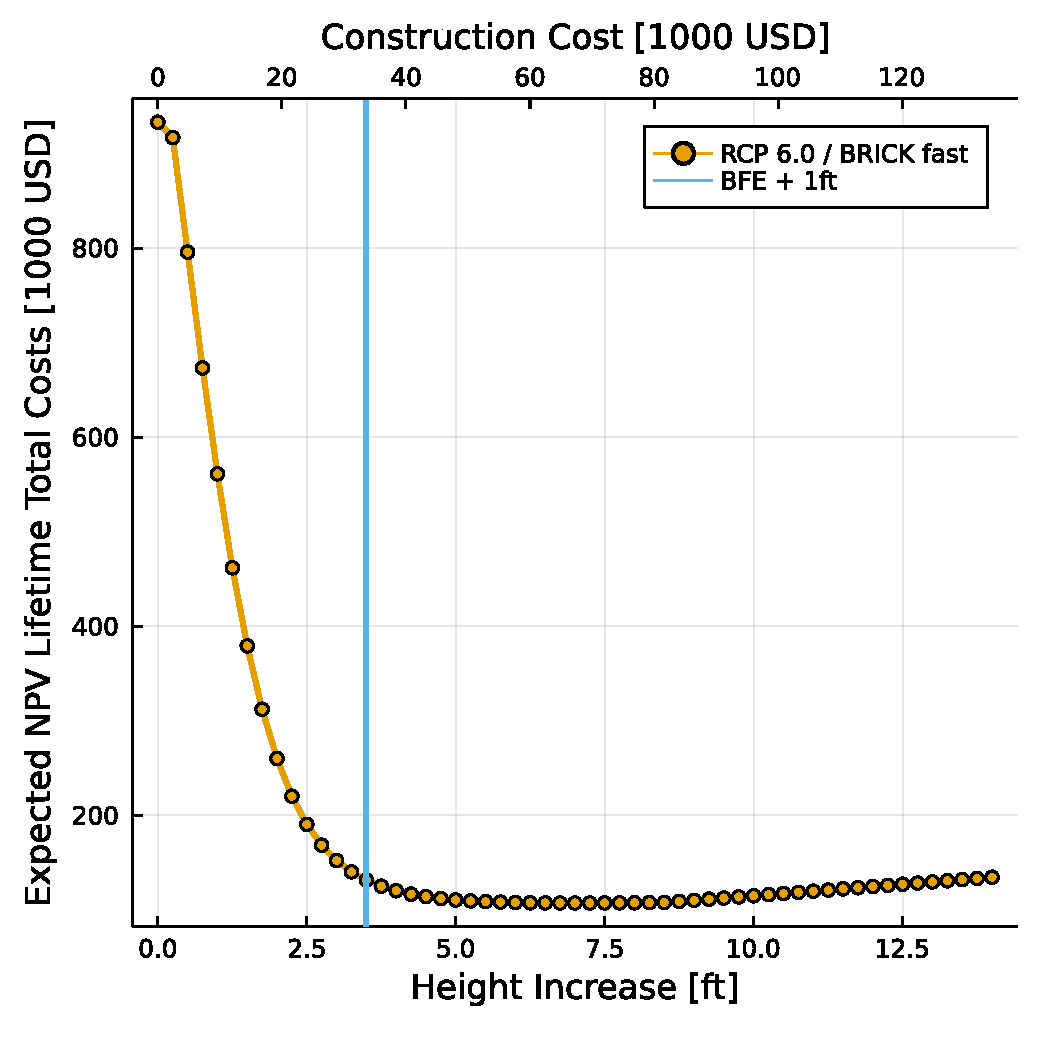
\includegraphics[width=0.475\textwidth]{5.5.pdf}%
            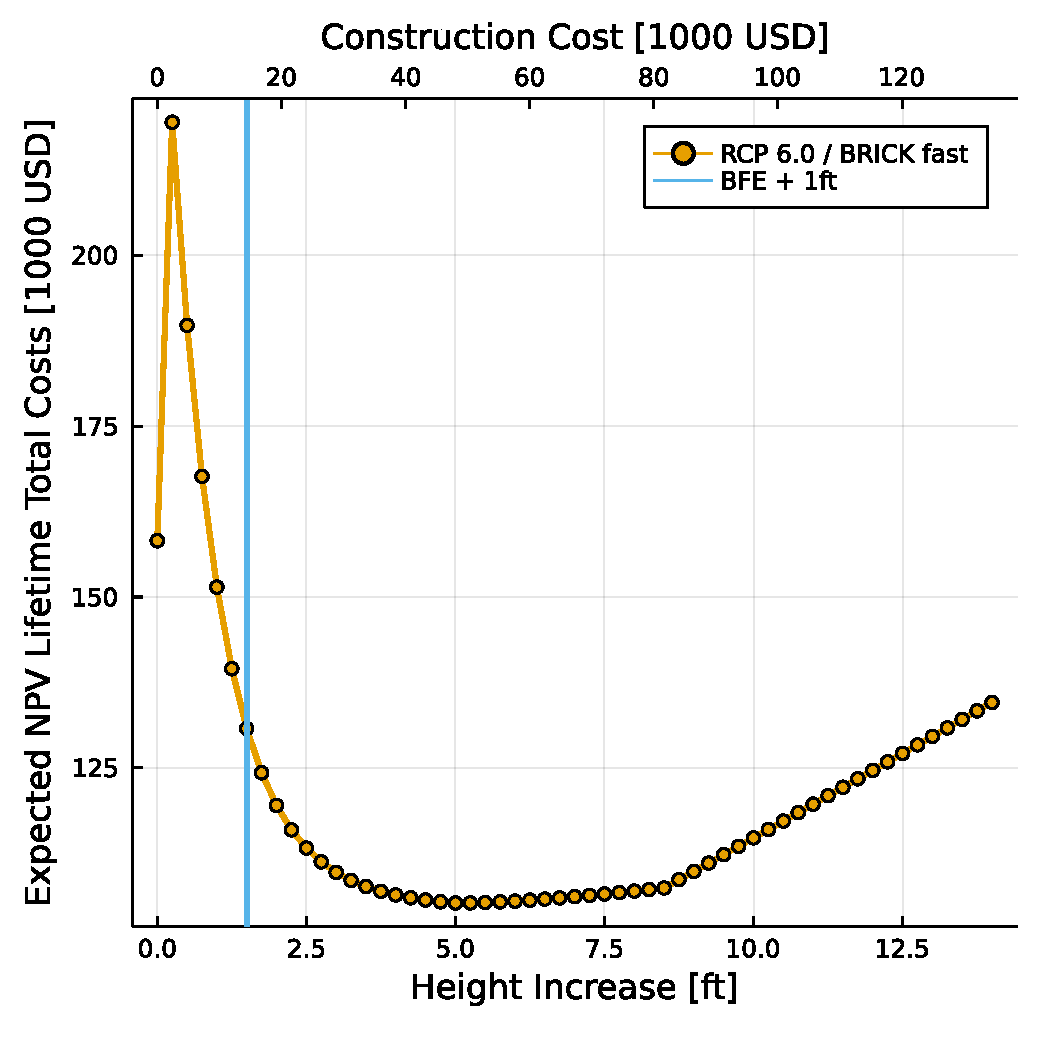
\includegraphics[width=0.475\textwidth]{7.5.pdf}
            \caption{
                Tradeoffs between construction cost and expected NPV lifetime costs for houses initially situated (L) \SI{2.5}{ft} and (R) \SI{0.5}{ft} below the \gls{bfe} under \gls{rcp} 6.0 with fast BRICK dynamics.
                Note $y$-axes are not equal.
            }
        \end{figure}
    \end{framed}
\end{block}